\chapter{Klassenbeschreibung Domain Layer}

Dieses Kapitel beschreibt die Klassen des Domain Layers, welche durch die vorigen Interfaces schon umrissen wurden. Das Diagramm \ref{domainentities} gibt eine Übersicht die Domain Entities der Anwendung und ist am Ende des Dokuments in größer angehängt.

%Model-----------------------------
\section{Domain Entities}

\begin{figure}[H]
\centering
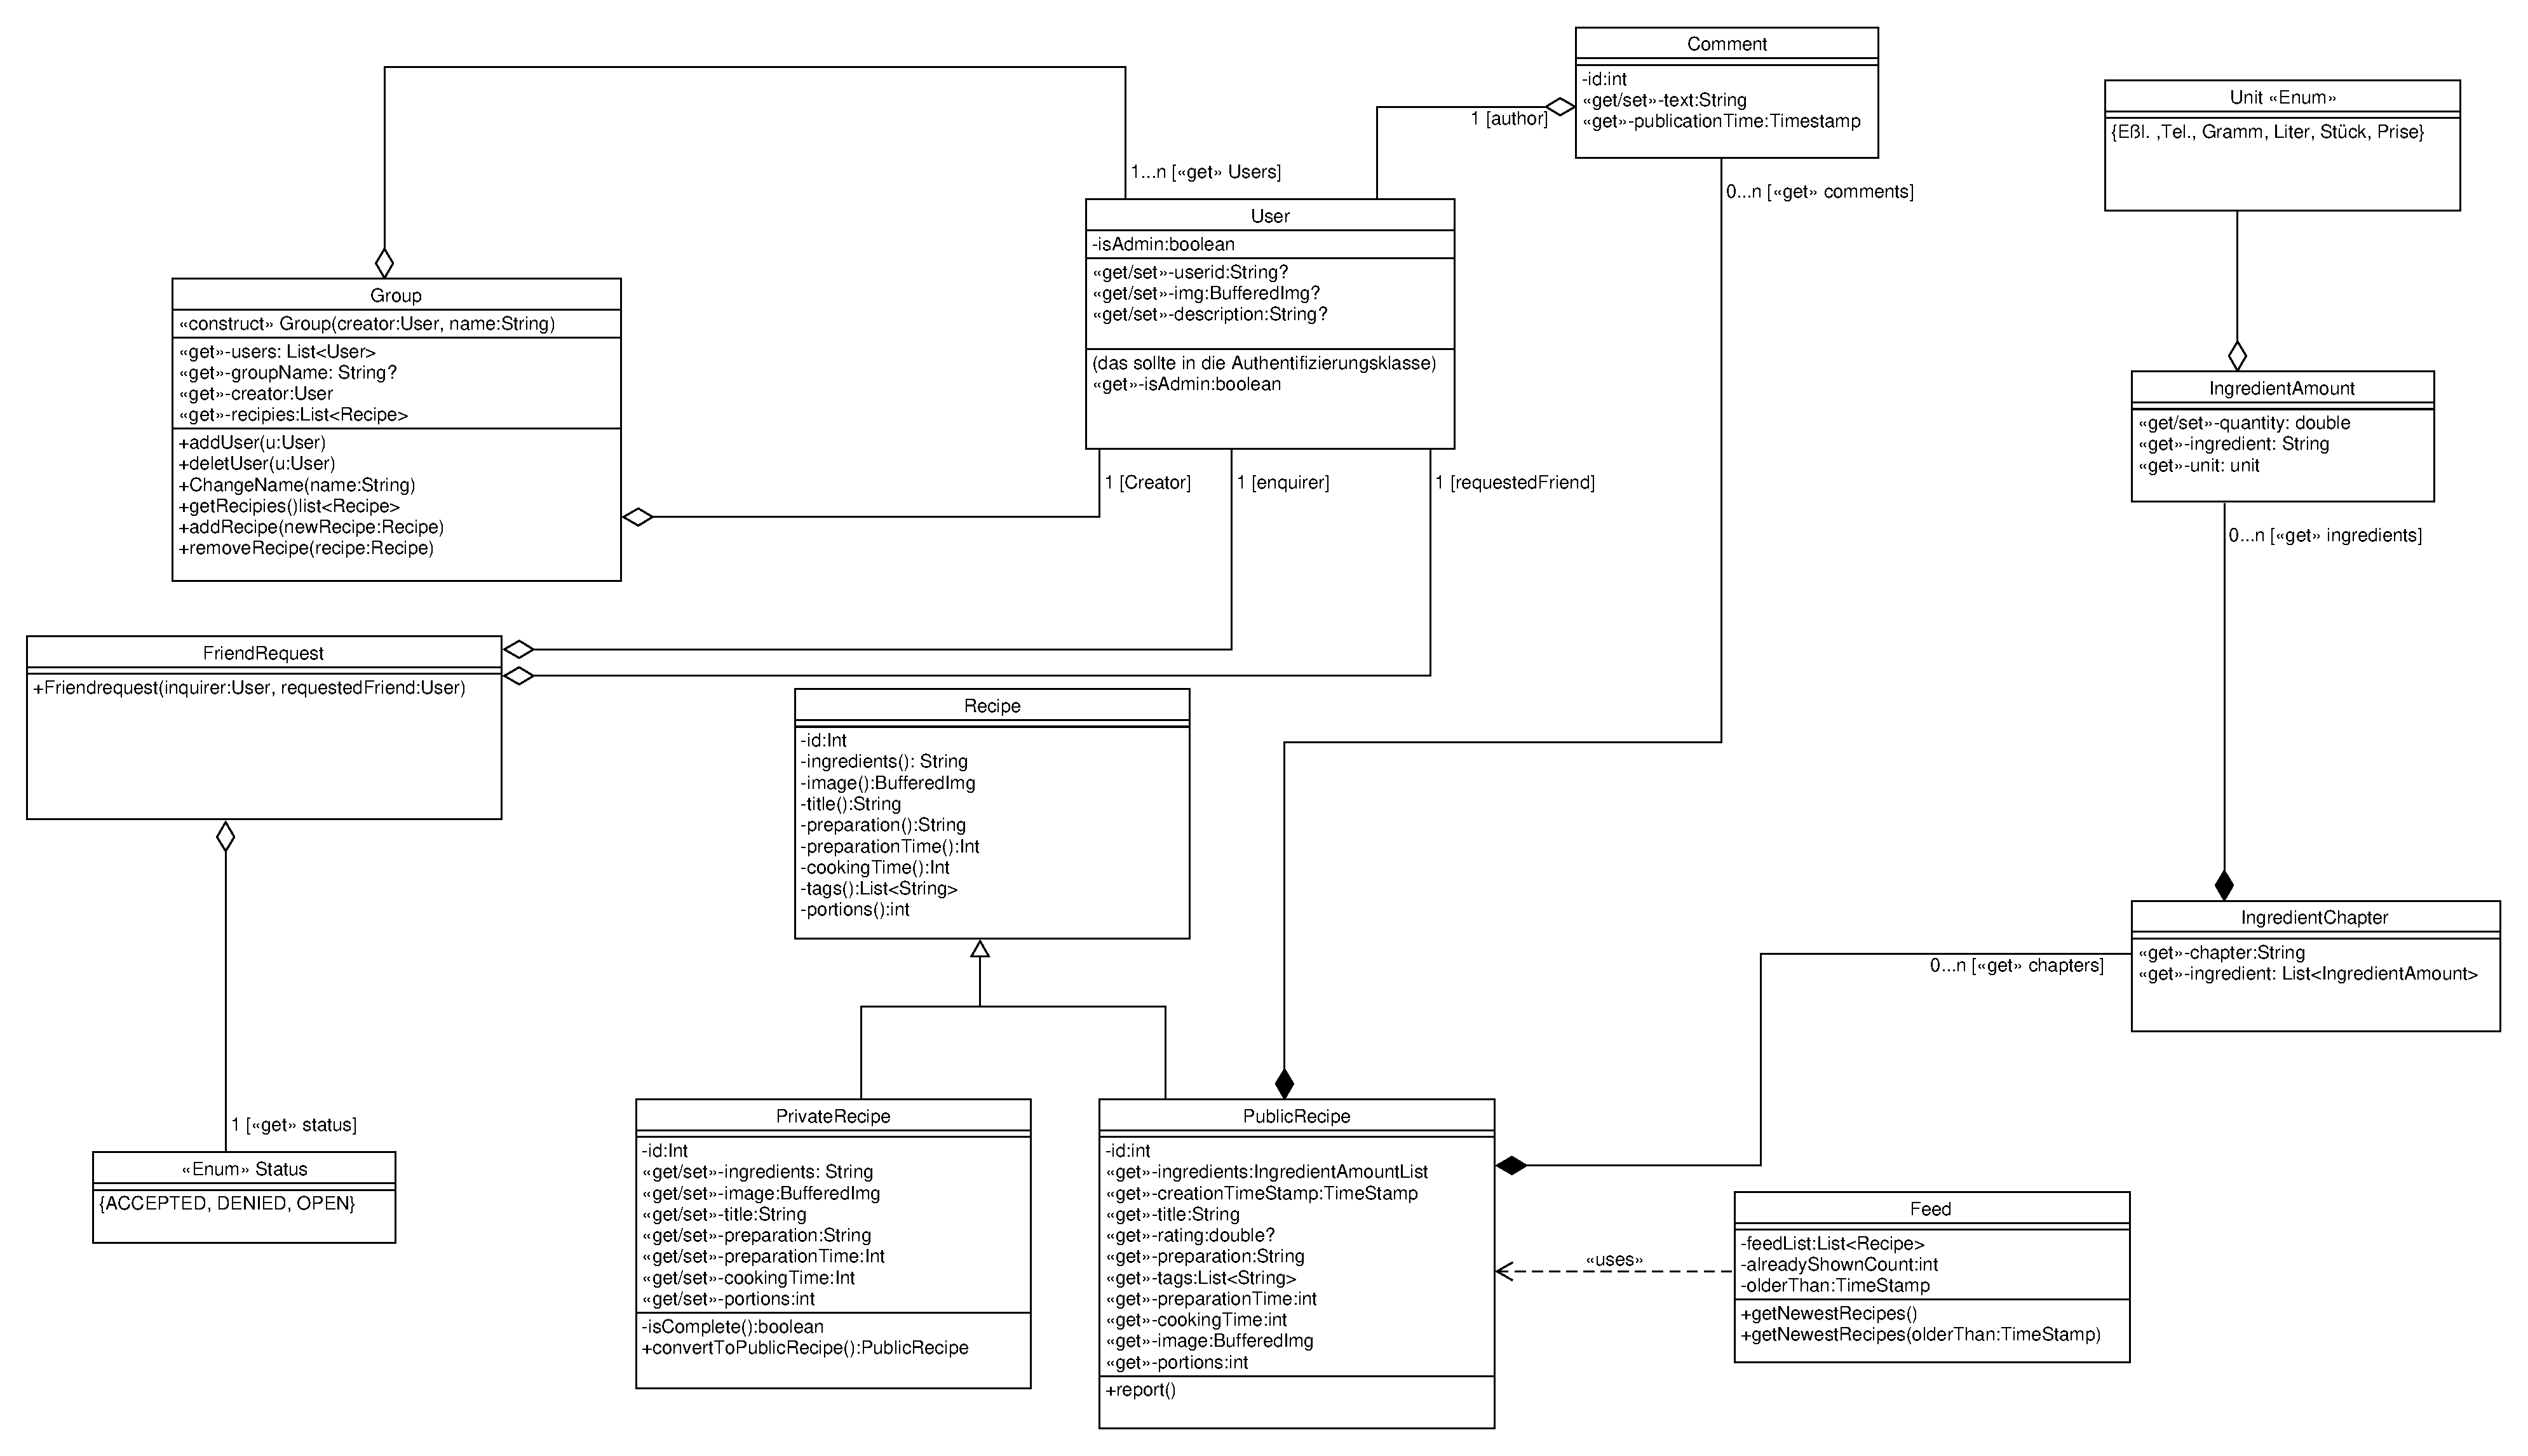
\includegraphics[width=0.7\textwidth]{pics/Domain_Entities_ueberarbeitet.pdf}%
\caption{Übersicht über die Domain Entities}%
\label{domainentities}%
\end{figure}

\subsection{User}
Die Klasse User beschreibt das Profil eines angemeldeten Nutzers.

\textbf{Attribute}
\begin{itemize}[nosep]
	\item iD:int \\ Eindeutige Identifikation des Profils 
	\item img:BufferedImage \\ Profilbild eines Profils
	\item description:String \\ textuelle Beschreibung des Profils
	\item isAdmin:boolean \\ beschreibt, ob ein Profil Adminrechte hat oder nicht
	\item email:String \\ E-Mail Adresse eines Profils, mit dem sich der Nutzer registriert
\end{itemize}
\subsubsection{Admin}
Die Klasse Admin erbt von der Klasse User und ist ein Singleton.Er hat die Aufgabe sich um gemeldete Rezepte, Gruppen und Nutzerprofile zu kümmern und diese zu verwalten. Das Singleton, welches hier verwendet wird, ist eine leichte Abweichung des Standards. Die Instanziierung des Admins muss zu Beginn einmal manuell gemacht werden. Der Singleton ist ein Erzeugungsmuster, wobei hier kein globaler Zugriff auf die Instanziierung gegeben wird.  Das Entwurfsmuster Einzelstück garantiert, dass es nur einen Admin geben kann.  Der Admin ist zudem noch dafür zuständig, falls jemand ein Problem mit der Applikation, oder ähnliches hat sich darum zu kümmern. Damit ist für die Nutzer die Möglichkeit geschaffen über den Admin als sichere Zwischeninstanz Probleme der Applikation zu handhaben.

\subsection{Group}
Diese Klasse beschreibt eine Gruppe von Freunden, in der private Rezepte geteilt werden können.

\textbf{Attribute}
\begin{itemize}[nosep]
	\item friendGroup:List<User> \\ Alle Nutzer die sich in der Gruppe befinden
	\item friendGroupName:String \\ Name der Gruppe
	\item creator:User \\ Ersteller der Gruppe
	\item recipes:List<Recipe> \\ Rezepte die in der Gruppe geteilt wurden
\end{itemize}

\subsection{<<Interface>> Recipe}
Dieses Interface beschreibt die Mindestfunktionalität, die ein Rezept haben muss, um angezeigt werden zu können.

\textbf{Methoden}
\begin{itemize}[nosep]
	\item getingredients():String \\ gibt textuelle Beschreibung der Zutaten zurück
	\item getimage():BufferedImage \\ gibt Bild des Rezeptes zurück
	\item gettitle():String \\ gibt Titel des Rezeptes zurück
	\item getpreparation():String \\ gibt textuelle Beschreibung der Zubereitung zurück
	\item getpreparationtime():int \\ gibt benötigte Zeit in Minuten der Zubereitung zurück
	\item getcookingTime():int \\ gibt benötigte Koch- bzw. Schmorzeit der Zubereitung zurück
	\item gettags():List<String> \\ gibt die dem Rezept gegebenen Tags zurück
	\item getportions():int \\ gibt die Anzahl Portionen, für die die Zutaten ausgelegt sind, zurück
\end{itemize}

\subsection{privateRecipe}
Diese Klasse beschreibt ein privates Rezept.

\textbf{Attribute}
\begin{itemize}[nosep]
	\item id:int \\ Falls ein privates Rezept schon veröffentlicht wurde, ist dies die id des zugehörigen öffentlichen Rezeptes
	\item ingredients:String \\ Textuelle Beschreibung der Zutaten
	\item title:String \\ Titel des privaten Rezeptes
	\item image:BufferedImage \\ Bild des Rezeptes
	\item preparation:String \\ Textuelle Beschreibung der Zubereitung
	\item preparationTime:int \\ Benötigte Zeit in Minuten der Zubereitung
	\item cookingTime:int \\ Benötigte Koch- bzw. Schmorzeit der Zubereitung
	\item tags:List<String> \\ Liste der dem Rezept gegebenen Tags
	\item portions:int \\ Anzahl Portionen, für die die Zutaten ausgelegt sind
\end{itemize}

\subsection{publicRecipe}
Diese Klasse beschreibt ein öffentliches Rezept.

\textbf{Attribute}
\begin{itemize}[nosep]
	\item id:int \\ Eindeutige Identifikation des öffentlichen Rezeptes
	\item ingredients:IngredientAmountList \\ Zutaten des Rezeptes
	\item creationTimeStamp:TimeStamp \\ Datum und Uhrzeit der Veröffentlichung
	\item title:String \\ Titel des Rezeptes
	\item rating:double \\ bewertung des Rezeptes
	\item preparation:String \\ Textuelle Beschreibung der Zubereitung
	\item tags:List<String> \\ Liste der dem Rezept gegebenen Tags
	\item preparationTime:int \\ Benötigte Zeit in Minuten der Zubereitung
	\item cookingTime:int \\ Benötigte Koch- bzw. Schmorzeit der
	\item image:BufferedImage \\ Bild des Rezeptes
	 Zubereitung
	\item comments:List<Comment> \\ Liste der dem Rezept gegebenen Kommentare
	\item portions:int \\ Anzahl Portionen, für die die Zutaten ausgelegt sind
\end{itemize}

\subsection{IngredientAmountList}
Diese Klasse beschreibt eine objektorientierte Zerlegung der Zutatenliste eines öffentlichen Rezeptes.

\textbf{Attribute}
\begin{itemize}[nosep]
	\item chapters:List<IngredientChapter> \\ Liste der Unterkapitel einer Zutatenliste eines Rezeptes
	\item portions:int \\ Anzahl an Portionen, für die das Rezept ausgelegt ist
\end{itemize}

\subsection{IngredientChapter}
Diese Klasse beschreibt ein Kapitel einer Zutatenliste eines Rezeptes.

\textbf{Attribute}
\begin{itemize}[nosep]
	\item chapter:String \\ Name des Kapitels
	\item ingredients:List<IngredientAmount> \\ Liste der Zutaten eines Kapitels
\end{itemize}

\subsection{IngredientAmount}
Diese Klasse beschreibt eine Zutat in einem Kapitel einer Zutatenliste.

\textbf{Attribute}
\begin{itemize}[nosep]
	\item ingredient:String \\ textuelle Beschreibung der Zutat
	\item unit:Unit \\ Einheit, in der die Zutat gemessen wird
	\item quantity:double \\ Anzahl an unit in der die Zutat benötigt wird
\end{itemize}

\subsection{Unit}
Diese Klasse beschreibt die Einheiten, in der Zutaten gemessen werden können.

\textbf{Attribute}
\begin{itemize}[nosep]
	\item Eßl \\ Einheit Esslöffel
	\item Tel \\ Einheit Teelöffel
	\item Liter \\ Einheit Liter
	\item g \\ Einheit Gramm
	\item kg \\ Einheit Kilogramm
\end{itemize}

%\subsection{PersonalUserData}
%Diese Klasse beinhaltet Informationen, die lokal für die Funktionalität der App benutzt werden.

%\textbf{Attribute}
%\begin{itemize}[nosep]
%	\item shoppingList:List<IngredientAmount> \\ Liste der Zutaten, die auf der Einkaufsliste Stehen
%	\item privateTags:List<String> \\ Liste der privaten Tags, die der User erstellt bzw. bearbeitet hat
%	\item recipeList:List<privateRecipe> \\ Liste der privaten Rezepte, die über einen Nutzer erstellt wurden
%	\item favoriteList:List<publicRecipe> \\ Liste an öffentlichen Rezepten, die über einen Nutzer favorisiert wurden
%	\item groups:List<Group> \\ Liste an Gruppen, in denen der Nutzer sich befindet
%	\item friends:List<User> \\ Liste an Benutzern, mit denen der Nutzer befreundet ist
%	\item accountData:User \\ Profildaten, des dem Account zugehörigen Profils
%\end{itemize}

\subsection{Feed}
Diese Klasse beschreibt den Feed an neuen Rezepten.

\textbf{Attribute}
\begin{itemize}[nosep]
	\item feedList:List<PublicRecipe> \\ Liste der neusten Rezepte
	\item alreadyShownCount:int \\ Anzahl der Rezepte, die von der App schon angezeigt wurden
	\item olderThan:TimeStamp \\ Datum und Uhrzeit, zu dem der Feed geladen wurde
\end{itemize}

\subsection{Comment}
Diese Klasse beschreibt einen Kommentar, der einem öffentlichen Rezept gegeben wurde.

\textbf{Attribute}
\begin{itemize}[nosep]
	\item id:int \\ Eindeutige Identifikation eines Kommentars
	\item text:String \\ Text des Kommentars
	\item publicationTime:TimeStamp \\ Datum und Uhrzeit, an dem ein Kommentar veröffentlicht wurde
	\item author:User \\ Verfasser des Kommentars
\end{itemize}

\section{Authentification}
Diese Klasse ist für die Authentifikation von einem Nutzer zuständig.

\textbf{Attribute}
\begin{itemize}[nosep]
	\item auth:FirebaseAuth \\Zugangspunkt zur Firebaseauthentifikation SDK
\end{itemize}
\textbf{Methoden}
\begin{itemize}[nosep]
	\item registrate(userId:String, email:String, password:String):void \\Ein neuer Nutzer wird auf Firebase registriert. Es wird die Nutzerid, Email und Passwort übergeben.
	\item login(email:String, password:String):void \\Logt einen Nutzer auf Firebase an. Es wird die Email und das Password übergeben.
	\item logout():void \\Meldet einen Nutzer in Firebase ab. 
	\item pwEdit(pw:String):void \\Ändert das Passwort eines Nutzers auf Firebase ab. Das neue Passwort wird übergeben.
	\item userIdEdit(userId:String):void \\Ändert den Nutzernamen eines Nutzers ab. Es wird der neue Nutzername übergeben.
	\item getToken():String \\Gibt den JWT-Token vom gerade angemeldeten Nutzer zurück.
\end{itemize}

\section{ImportExport}

\begin{lstlisting}
importExport.shareRecipe(Recipe) : void
importExport.parseIntent(Intent) : privateRecipe
\end{lstlisting}

Kriterium \textbf{W7} der zu entwickelten App definiert die Funktionalität, Rezepte teilen und importieren zu können. 

Das Android Framework sieht dafür Intents und  Intentfilter vor. 
Das oben beschriebene Interface kapselt dafür Funktionalität. 
Die Klasse, die das Interface implementiern, wird nun beschrieben.

\subsection{Export}
Wird importExport.shareRecipe() aufgerufen, wird aus dem als Parameter übergebenen Rezept ein Textintent generiert und an das Framework übergeben. 

Beispielcode:

\begin{lstlisting}
// Create the text message with a string
val sendIntent = Intent().apply {
    action = Intent.ACTION_SEND
    putExtra(Intent.EXTRA_TEXT, textMessage)
    type = "text/plain"
}
\end{lstlisting}


Das Android Framework kümmert sich dann darum, ein Dialogfenster mit kompatiblen Apps anzuzeigen, in denen
das Rezept geteilt werden kann. 

\begin{figure}[H]
\centering
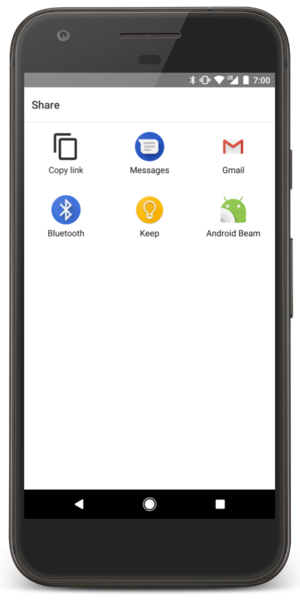
\includegraphics[width=0.2\textwidth]{pics/intentchoser.png}%
\caption{Dialogfenster zum Auswählen der App, die den Intent erhält \cite{AndroidArchitectureComponents}}%
\label{choseapp}%
\end{figure}

\begin{figure}[H]
\centering
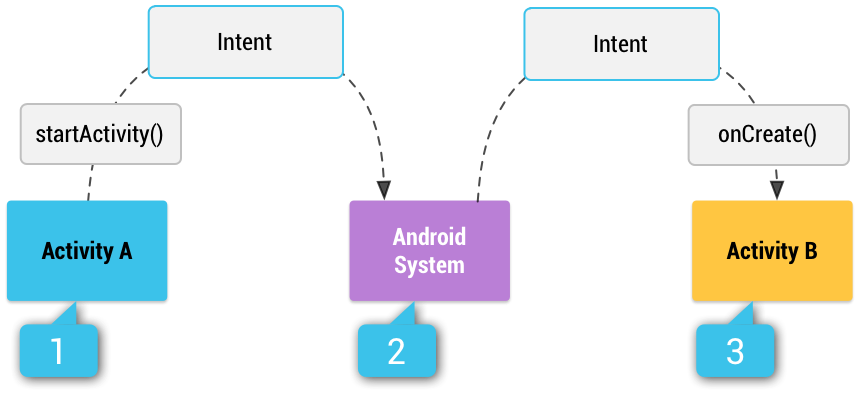
\includegraphics[width=0.7\textwidth]{pics/android_arch_intentfilter.png}%
\caption{Schaubild, Übergabe von Intents zwischen Androidapps \cite{AndroidArchitectureComponents}}%
\label{arch_intentfilter}%
\end{figure}


\subsection{Import} 
Zum Importieren registriert die App Intentfilter mit einem <intent-filter> element in der Manifestdatei. Jeder Intentfilter spezifisiert den Typ einer Kategorie von Intents, die die App akzeptiert. So kann die App sich für HTML URLs und Text als Empfänger von Intents registrieren. Daraufhin wird vom System, die Activity aufgerufen, die dafür im Manifest registriert ist. Die Activity und das zugehörige ViewModel, was  dieses Intent dann erhält, kann dann die Methode parseIntent() aufrufen. 
Diese dient dann dazu, aus dem Intent ein privates Rezept zu parsen. 
